\documentclass[notes,11pt, aspectratio=169, xcolor=table]{beamer}

\usepackage{pgfpages}
% These slides also contain speaker notes. You can print just the slides,
% just the notes, or both, depending on the setting below. Comment out the want
% you want.
\setbeameroption{hide notes} % Only slide
%\setbeameroption{show only notes} % Only notes
%\setbeameroption{show notes on second screen=right} % Both


\newtheorem{proposition}{Proposition}
\newcommand{\blue}[1]{\textcolor{blue}{#1}}
\newcommand{\white}[1]{\textcolor{white}{#1}}

\usepackage{helvet}
\usepackage[default]{lato}
\usepackage{array}
\usepackage{tikz}
\usetikzlibrary{shapes.geometric}
\usepackage{pgfplots}
\usetikzlibrary{patterns, pgfplots.fillbetween}
\usepackage{graphicx}
\usepackage{verbatim}
\setbeamertemplate{note page}{\pagecolor{yellow!5}\insertnote}
\usetikzlibrary{positioning}
\usetikzlibrary{snakes}
\usetikzlibrary{calc}
\usetikzlibrary{arrows}
\usetikzlibrary{decorations.markings}
\usetikzlibrary{shapes.misc}
\usetikzlibrary{matrix,shapes,arrows,fit,tikzmark}
\usepackage{amsmath}
\usepackage{mathpazo}
\usepackage{hyperref}
\usepackage{lipsum}
\usepackage{multimedia}
\usepackage{graphicx}
\usepackage{multirow}
\usepackage{graphicx}
\usepackage{dcolumn}
\usepackage{bbm}
\usepackage{emoji}
\usepackage[style=authoryear,sorting=nyt,uniquename=false]{biblatex}

\addbibresource{references.bib} 

\newcolumntype{d}[0]{D{.}{.}{5}}

\def\@@mybluebox[#1][#2]#3{
    \sbox\mytempbox{#3}%
    \mytemplen\ht\mytempbox
    \advance\mytemplen #1\relax
    \ht\mytempbox\mytemplen
    \mytemplen\dp\mytempbox
    \advance\mytemplen #2\relax
    \dp\mytempbox\mytemplen
    \colorbox{myblue}{\hspace{1em}\usebox{\mytempbox}\hspace{1em}}}


\usepackage{changepage}
\usepackage{appendixnumberbeamer}
\newcommand{\beginbackup}{
   \newcounter{framenumbervorappendix}
   \setcounter{framenumbervorappendix}{\value{framenumber}}
   \setbeamertemplate{footline}
   {
     \leavevmode%
     \hline
     box{%
       \begin{beamercolorbox}[wd=\paperwidth,ht=2.25ex,dp=1ex,right]{footlinecolor}%
%         \insertframenumber  \hspace*{2ex} 
       \end{beamercolorbox}}%
     \vskip0pt%
   }
 }
\newcommand{\backupend}{
   \addtocounter{framenumbervorappendix}{-\value{framenumber}}
   \addtocounter{framenumber}{\value{framenumbervorappendix}} 
}


\usepackage{graphicx}
\usepackage[space]{grffile}
\usepackage{booktabs}

% These are my colors -- there are many like them, but these ones are mine.
\definecolor{blue}{RGB}{0,114,178}
\definecolor{red}{RGB}{213,94,0}
\definecolor{yellow}{RGB}{240,228,66}
\definecolor{green}{RGB}{0,158,115}

\hypersetup{
  colorlinks=false,
  linkbordercolor = {white},
  linkcolor = {blue}
}


%% I use a beige off white for my background
\definecolor{MyBackground}{RGB}{255,253,218}

%% Uncomment this if you want to change the background color to something else
%\setbeamercolor{background canvas}{bg=MyBackground}

%% Change the bg color to adjust your transition slide background color!
\newenvironment{transitionframe}{
  \setbeamercolor{background canvas}{bg=yellow}
  \begin{frame}}{
    \end{frame}
}

\setbeamercolor{frametitle}{fg=blue}
\setbeamercolor{title}{fg=blue}
\setbeamertemplate{footline}[frame number]
\setbeamertemplate{navigation symbols}{} 
\setbeamertemplate{itemize items}{-}
\setbeamercolor{itemize item}{fg=blue}
\setbeamercolor{itemize subitem}{fg=blue}
\setbeamercolor{enumerate item}{fg=blue}
\setbeamercolor{enumerate subitem}{fg=blue}
\setbeamercolor{button}{bg=MyBackground,fg=blue,}



% If you like road maps, rather than having clutter at the top, have a roadmap show up at the end of each section 
% (and after your introduction)
% Uncomment this is if you want the roadmap!
% \AtBeginSection[]
% {
%    \begin{frame}
%        \frametitle{Roadmap of Talk}
%        \tableofcontents[currentsection]
%    \end{frame}
% }
\setbeamercolor{section in toc}{fg=blue}
\setbeamercolor{subsection in toc}{fg=red}
\setbeamersize{text margin left=1em,text margin right=1em} 

\newenvironment{wideitemize}{\itemize\addtolength{\itemsep}{10pt}}{\enditemize}

\usepackage{environ}
\NewEnviron{videoframe}[1]{
  \begin{frame}
    \vspace{-8pt}
    \begin{columns}[onlytextwidth, T] % align columns
      \begin{column}{.58\textwidth}
        \begin{minipage}[t][\textheight][t]
          {\dimexpr\textwidth}
          \vspace{8pt}
          \hspace{4pt} {\Large \sc \textcolor{blue}{#1}}
          \vspace{8pt}
          
          \BODY
        \end{minipage}
      \end{column}%
      \hfill%
      \begin{column}{.42\textwidth}
        \colorbox{green!20}{\begin{minipage}[t][1.2\textheight][t]
            {\dimexpr\textwidth}
            Face goes here
          \end{minipage}}
      \end{column}%
    \end{columns}
  \end{frame}
}

\title[]{International Trade: Lecture 6}
\subtitle[]{Empirics of Comparative Advantage}
\author[Góes]
{Carlos Góes\inst{1}}
\date{Fall 2025}
\institute[GWU]{\inst{1} George Washington University }



\begin{document}

%%% TIKZ STUFF
\tikzset{   
        every picture/.style={remember picture,baseline},
        every node/.style={anchor=base,align=center,outer sep=1.5pt},
        every path/.style={thick},
        }
\newcommand\marktopleft[1]{%
    \tikz[overlay,remember picture] 
        \node (marker-#1-a) at (-.3em,.3em) {};%
}
\newcommand\markbottomright[2]{%
    \tikz[overlay,remember picture] 
        \node (marker-#1-b) at (0em,0em) {};%
}
\tikzstyle{every picture}+=[remember picture] 
\tikzstyle{mybox} =[draw=black, very thick, rectangle, inner sep=10pt, inner ysep=20pt]
\tikzstyle{fancytitle} =[draw=black,fill=red, text=white]
%%%% END TIKZ STUFF



%----------------------------------------------------------------------%
%-------------------       TITLE PAGE       ---------------------------%
%----------------------------------------------------------------------%





%----------------------------------------------------------------------%






%----------------------------------------------------------------------%
%----------------------------------------------------------------------%

%----------------------------------------------------------------------%
\frame{\titlepage}
\addtocounter{framenumber}{-1}
%----------------------------------------------------------------------%



%----------------------------------------------------------------------%
%----------------------------------------------------------------------%


\begin{frame}{Testing the Ricardian Model}
    \begin{wideitemize}
        \item Ricardo provides a central model that underpins our intuitions about international trade

        \item<2-> But very little has been done to confront its predictions with the data

        \item<3-> \blue{Challenge (i):} autarky productivities and prices are unobserved

        \item<4-> If we assume productivities are fixed, we can ``infer'' autarky prices as function of technology and tastes

        \item<5-> Is that trivial?

        \item<5-> \blue{Challenge (ii):} for a long time, the Ricardian model was purely bilateral \\ 
        \qquad (changes with Eaton-Kortum, but that we do not cover it)

    \end{wideitemize}
\end{frame}

\begin{frame}{Some problems}
    \begin{wideitemize}
        \item Complete specialization

        \begin{itemize}
            \item Model predicts only one country ($H$ or $F$) supplies a given market

            \item<2-> But that does seem to agree with the data in the level of aggregate we have
                \qquad \textcolor{gray}{(at the end of the semester, we will cover interindustry trade)}

            \item<3-> Even if we find non-produced goods, how can we measure productivity autarky prices?
        \end{itemize}

        \item<4-> It is really hard to compare sectoral productivity across countries

        \begin{itemize}
            \item<4-> If we go by value, a Norwegian barber is 50x more productive than an Indian barbe
            \item<5-> Is that really true?
            \item<6-> Labor markets reflect opportunity costs
        \end{itemize}

        \item<7-> Model is very simple to begin with:
        \begin{itemize}
            \item<7-> In practice there multiple factors
            \item<8-> Intermediate goods, supply chain linkages
            \item<9-> Of course that model will not encompass all of the data
        \end{itemize}

        \item<10-> Question: can the most important mechanism be right?

    \end{wideitemize}
\end{frame}



\begin{frame}{Early tests}
    \begin{wideitemize}
        \item MacDougall (1951) used relative productivity measures to ``test'' Ricardian

        \item<2-> With 2 countries in the world (UK an USA) then each country will:

        \begin{blockquote}
            “export those goods for which the ratio of its output per worker to that of the other country exceeds the ratio of its money wage rate to that of the other country.”
        \end{blockquote}

        \item<3-> lots relative labor productivities (US:UK) against relative exports to the entire world (US:UK)

        \begin{itemize}
            \item 2 × 2 Ricardian intuition suggests that this should be upward-sloping.
            \item Nothing about how much a country will export. 
        \end{itemize}
        
    \end{wideitemize}
\end{frame}

\begin{frame}{MacDougall's chart}
    \begin{figure}
        \centering
        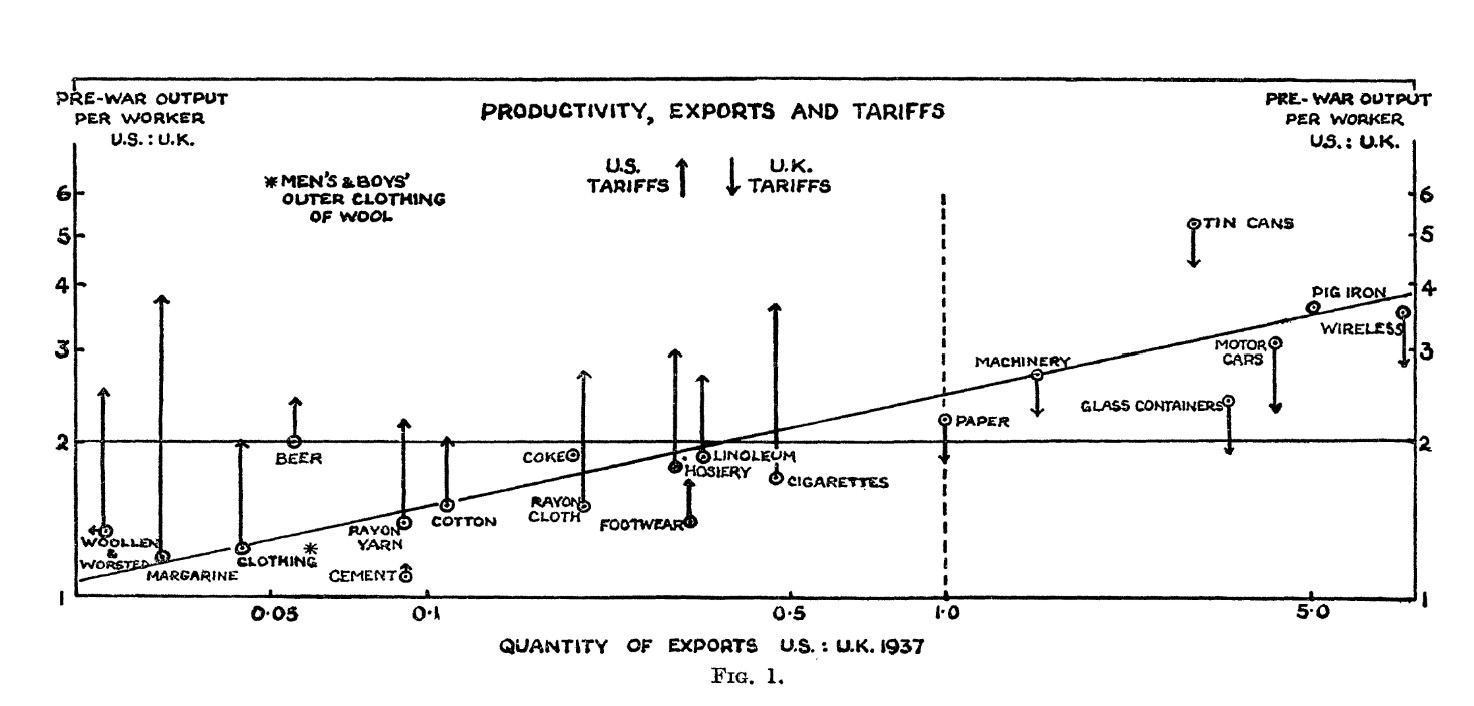
\includegraphics[width=0.9\linewidth]{figs/MacDougall1.jpg}
        \caption{Source: \href{https://www.jstor.org/stable/pdf/2226976.pdf}{MacDougall (1951)} }
        \label{fig:macdouall}
    \end{figure}
\end{frame}

\begin{frame}{...then replicated other times}
    \begin{figure}
        \centering
        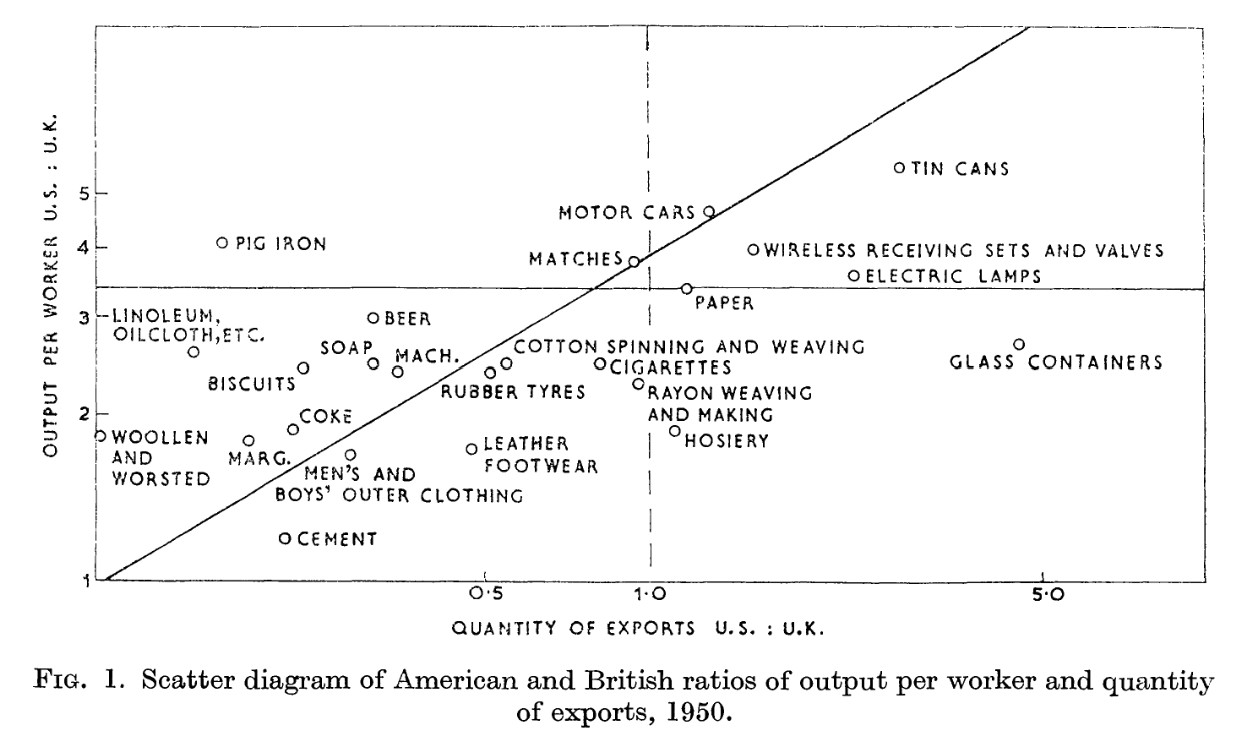
\includegraphics[width=0.75\linewidth]{figs/stern1962.jpg}
        \caption{Source: \href{https://www.jstor.org/stable/2661740?seq=1}{Stern (1962)} }
        \label{fig:stern}
    \end{figure}
\end{frame}

\begin{frame}{Tying the model to the data}

\begin{wideitemize}
    \item<1-> \blue{Question}: which country has a comparative advantage in good $g$ if $\frac{w_H}{w_F} \le  \frac{a_{F,g}}{a_{H,g}}$?

    \item<2-> Production only if cheaper to produce domestically than to import goods, i.e.:

    \begin{equation*}
        w_H a_{H,g} \le w_F a_{F,g} \text{ or, equivalently, if } \frac{w_H}{w_F} \le  \frac{a_{F,g}}{a_{H,g}}
    \end{equation*}

    \item<3-> Countries are expected to export goods in which they have high productivity (low unit labor requirements)
\end{wideitemize}

    
\end{frame}

\begin{frame}{Tying the model to the data}

\begin{wideitemize}
    \item<1-> Golub and Hsieh (2000) take this approach to test the Ricardian theory

    \item<2-> Recall we are expanding from the bilateral Ricardian model, so we are comparing two countries: $i$ and $j$.

    \item<3-> Then we could run the following regressions to test predictions:

    \begin{eqnarray*}
        \ln \left( \frac{X_{i}^k}{X_{j}^k} \right) &=& \alpha_1 + \beta_1 \ln \left(\frac{a_{j}^k}{a_{i}^k} \right) + \varepsilon_1^k \\
        \ln \left( \frac{X_{i\to j}^k}{X_{j \to i}^k} \right) &=& \alpha_2 + \beta_2 \ln \left(\frac{a_{j}^k}{a_{i}^k} \right) + \varepsilon_2^k 
    \end{eqnarray*}
    where $X_{i}^k$ are total exports of good $k$ in country $i$; and $X_{i\to j}^k$ are bilateral exports from $i$ to $j$.
    
    
\end{wideitemize}

    
\end{frame}

\begin{frame}{Golub and Hsieh (2000)}

    \begin{eqnarray*}
        \ln \left( \frac{X_{i}^k}{X_{j}^k} \right) &=& \alpha_1 + \beta_1 \ln \left(\frac{a_{j}^k}{a_{i}^k} \right) + \varepsilon_1^k \\
        \ln \left( \frac{X_{i\to j}^k}{X_{j \to i}^k} \right) &=& \alpha_2 + \beta_2 \ln \left(\frac{a_{j}^k}{a_{i}^k} \right) + \varepsilon_2^k 
    \end{eqnarray*}
    
    \begin{wideitemize}

    \item<1-> How is this related to Ricardian theory?

    \item<2-> In which does it differ importantly from the theory?

    \item<3-> The intuition of the Ricardian model suggests that $\beta_1 > 0$ and $\beta_2 > 0$. \\
        \qquad (countries should export goods they are most productive in)
    
    \item<4-> But we are extrapolating from a 2x2 model to multicountry data; no obvious way to interpret the results. \\
        \qquad (model predicts \textit{full specialization})

\end{wideitemize}

\end{frame}


\begin{frame}{Results are consistent with the Ricardian intuition}
    \begin{figure}
        \centering
        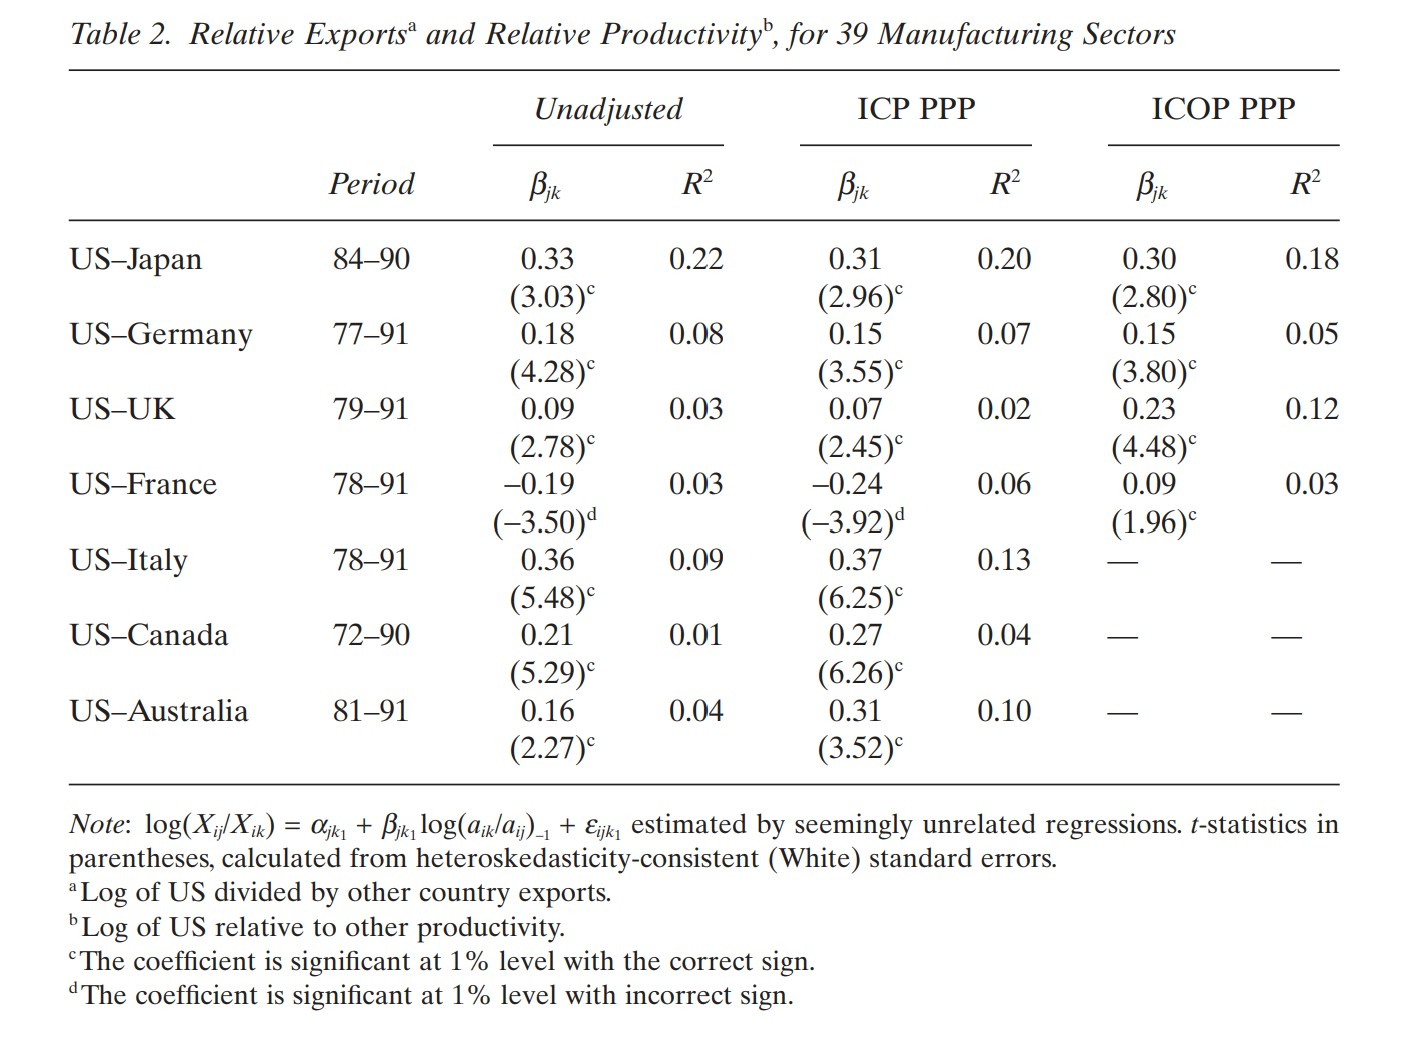
\includegraphics[width=0.6\linewidth]{figs/golub-hsieh.jpg}
        \caption{Source: \href{https://onlinelibrary.wiley.com/doi/epdf/10.1111/1467-9396.00217}{Golub and Hsieh (2000)} }
        \label{fig:golub}
    \end{figure}
\end{frame}

\begin{frame}{Results are consistent with the Ricardian intuition}
    \begin{figure}
        \centering
        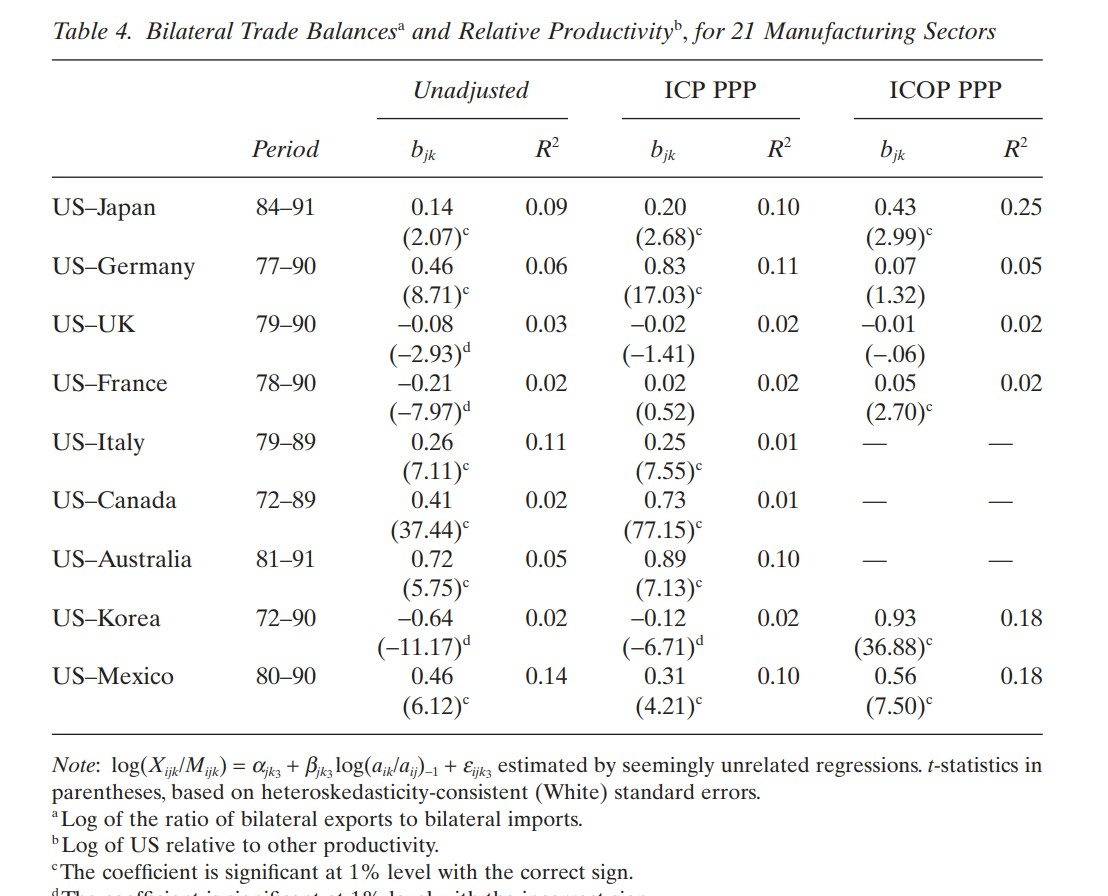
\includegraphics[width=0.5\linewidth]{figs/golub-hsieh3.jpg}
        \caption{Source: \href{https://onlinelibrary.wiley.com/doi/epdf/10.1111/1467-9396.00217}{Golub and Hsieh (2000)} }
        \label{fig:golub2}
    \end{figure}
\end{frame}

\begin{frame}{Caveats...}
\begin{wideitemize}
    \item Results are consistent with the Ricardian intuition...

    \item ...but there are some caveats.

    \item The main issue is that it takes a leap of faith to go from a 2x2 model to cross-country evidence

    \item<2-> Empirically, measuring $a_i^k$ is not easy.

    \begin{itemize}
        \item<2-> Comparing different currencies.
        \item<3-> Market exchange rates are likely to be misleading
        \item<4-> PPP exchange rates  used instead
        \item<5-> Think of this as ``Big Mac index''
    \end{itemize}
\end{wideitemize}

\end{frame}

\begin{frame}{Big Mac Index}
    \begin{wideitemize}
        \item A Big Mac is identical all over the world... \vspace{10pt}
        \begin{center}
        \onslide<2->{\Large \textit{Two all beef patties, special sauce, lettuce, cheese, pickles, onions on a sesame seed bun} \scriptsize (\href{https://www.youtube.com/watch?v=yEBCV0ic6Tc}{original jingle})}
        \end{center}

        \item<3-> If a Big Macs could be teleported to the point of sale, they would be produced in the place where they are cheapest

        \item<4-> Why do prices differ
        \begin{itemize}
            \item Labor is not mobile across countries
            \item Other factors of production (rent) are immobile
            \item You cannot ship a burger long distance
        \end{itemize}

    \end{wideitemize}
\end{frame}

\begin{frame}{Big Mac Index}
    \begin{figure}
        \centering
        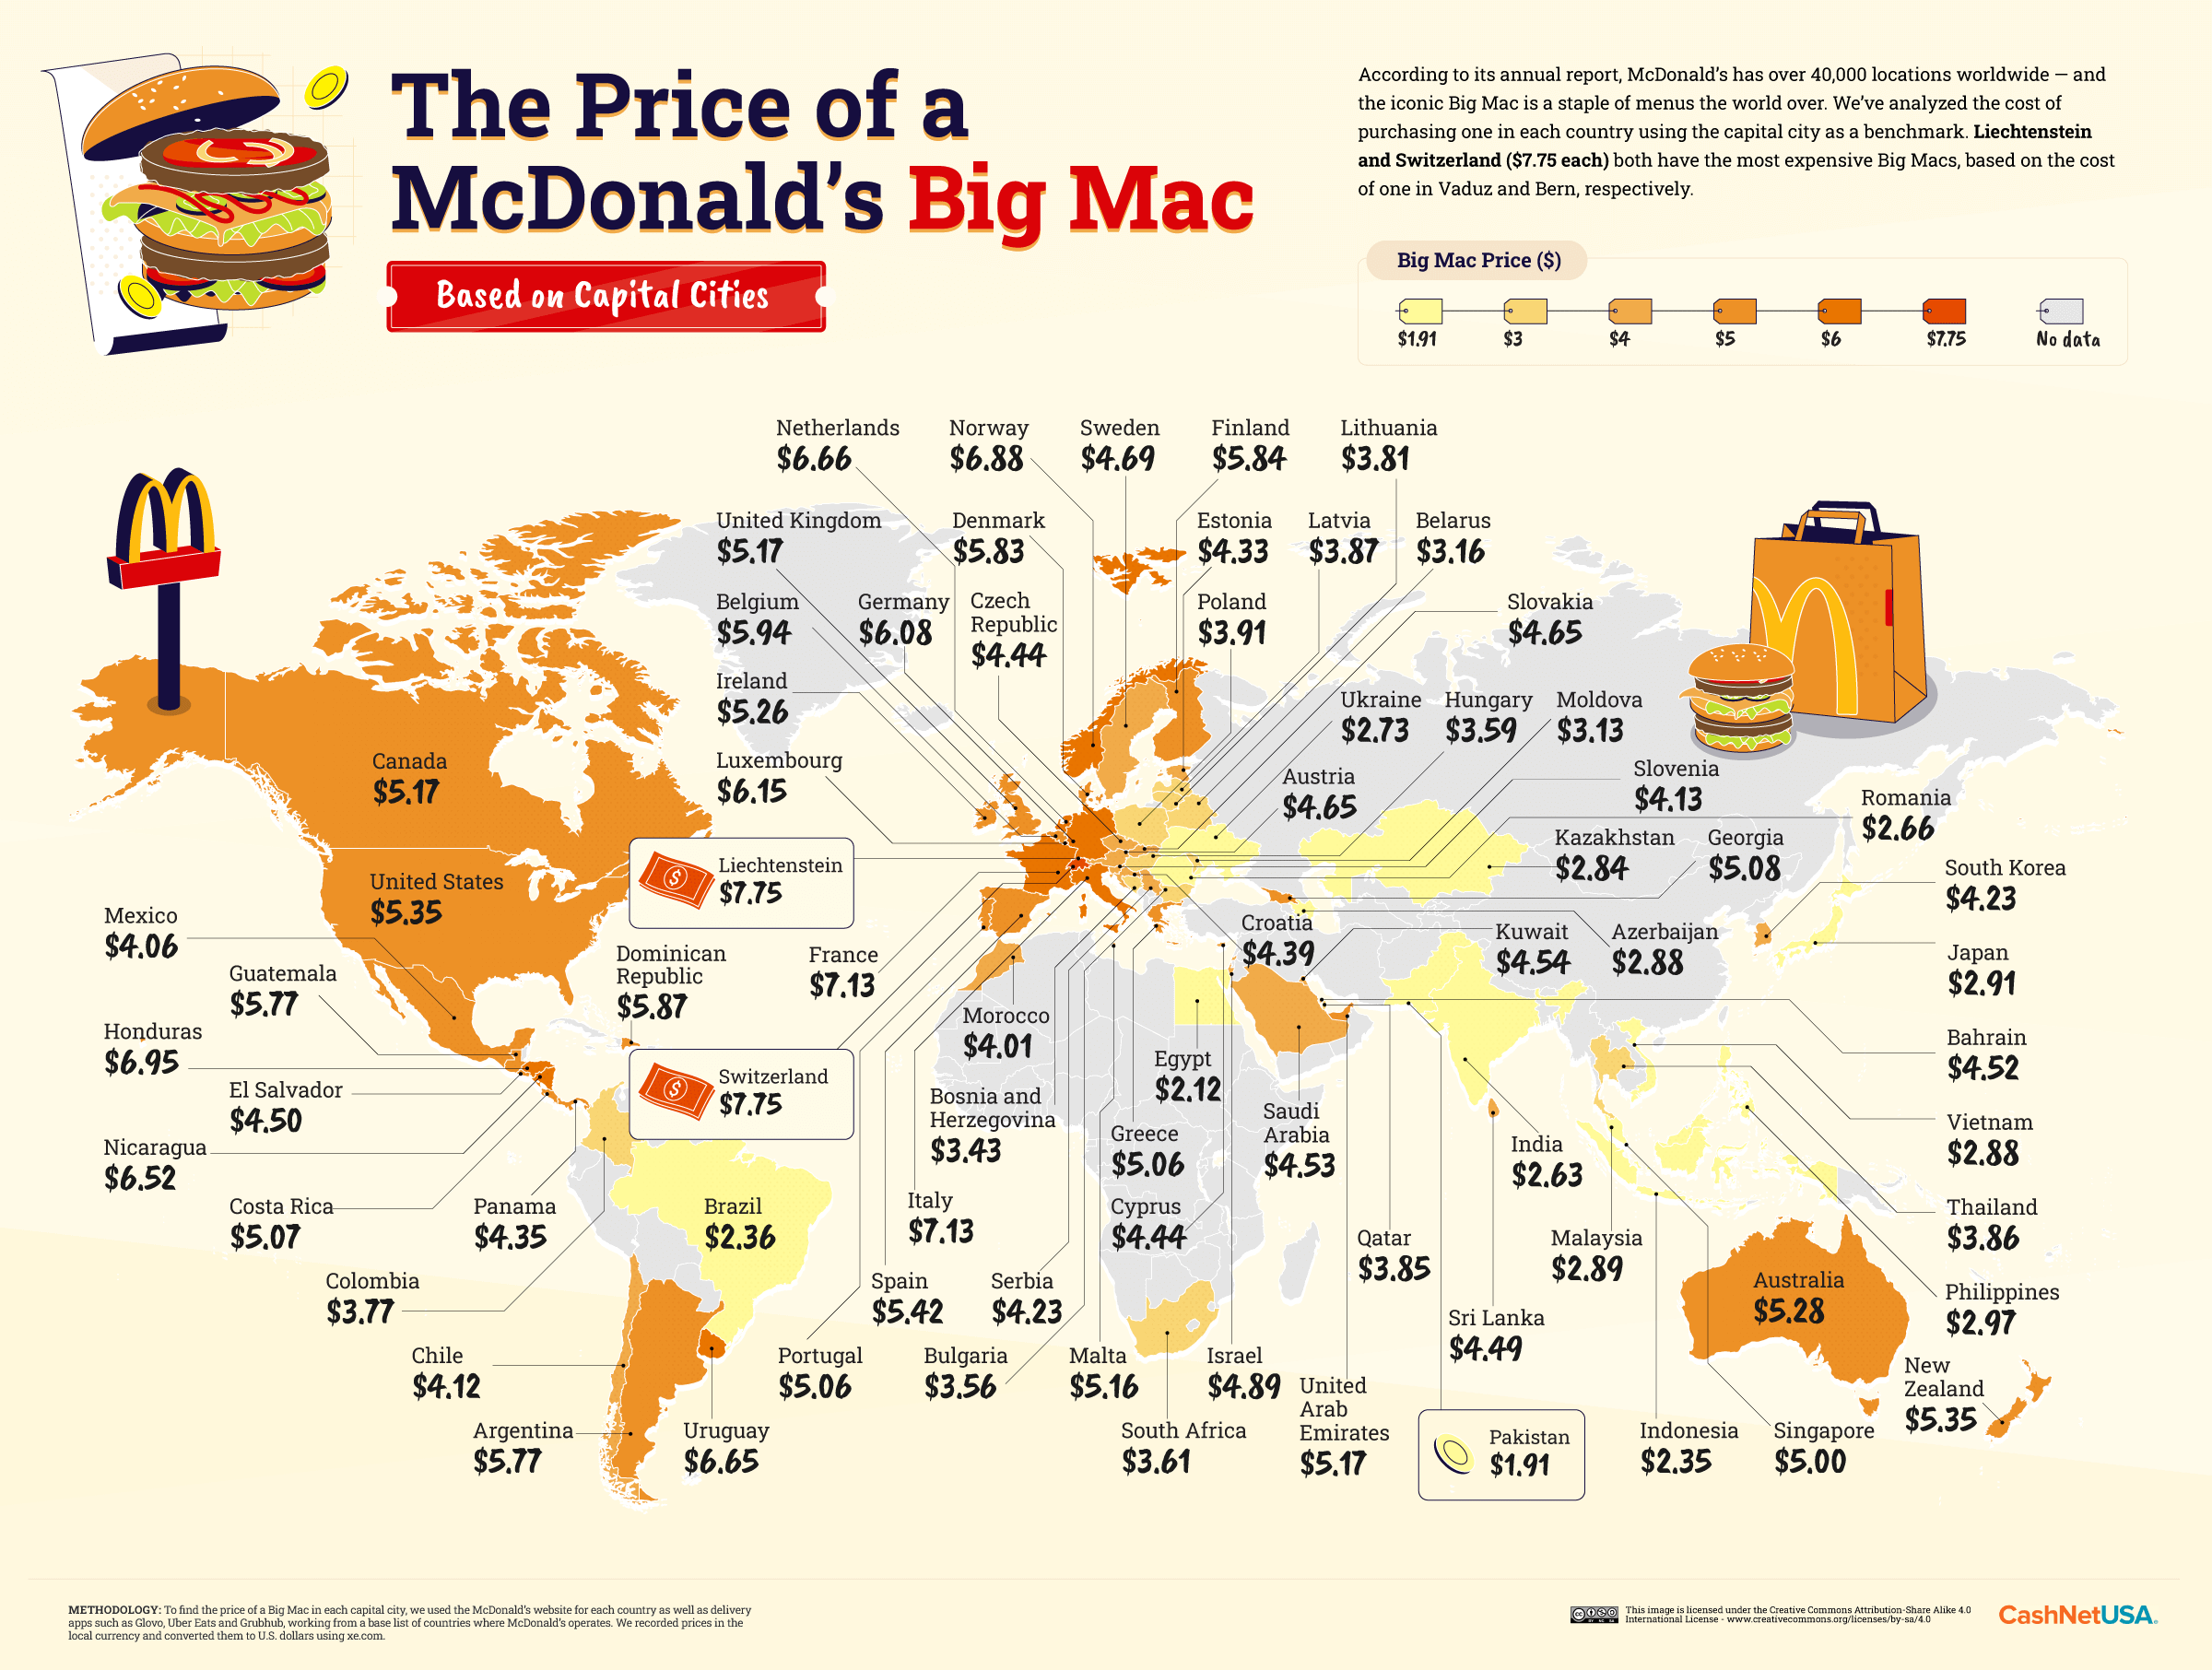
\includegraphics[width=0.65\linewidth]{figs/01_The-Price-of-McDonalds-Big-Mac_World-Map.png}
    \end{figure}
\end{frame}


\begin{frame}{Balassa Samuelson Effect}
    \begin{figure}
        \centering
        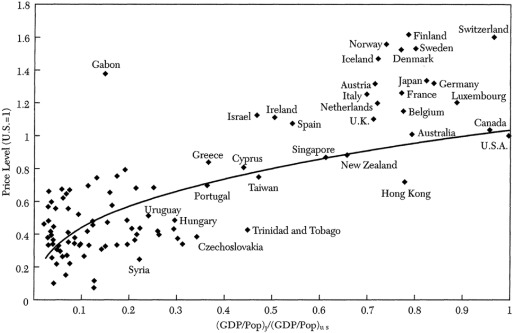
\includegraphics[width=0.65\linewidth]{figs/balassa-samuelson.jpg}
        \caption{Balassa Samuelson Effect: Goods and Services are more expensive in richer countries \href{https://scholar.harvard.edu/files/rogoff/files/51_jel1996.pdf}{(Rogoff, 1996)}}
    \end{figure}
\end{frame}


\begin{frame}{Purchasing Power Parity}
    \begin{wideitemize}
        \item Prices are sistematically higher in richer countries:
        \begin{itemize}
            \item Nontradables reflect domestic wages and technology
            \item Service economy (largely nontradable) more important
        \end{itemize}


        \item \href{https://www.worldbank.org/en/programs/icp}{World Bank's International Comparison Program} collects data on prices for many goods across countries to create benchmarks 

        \item \blue{Output:} How much is a dollar worth in each country (US is the benchmark)

        \item When comparing productivities and incomes, economists often adjust for overall price levels

        \item \blue{Intuition}:
            \begin{itemize}
                \item Inflation adjustment corrects for price differences across time (e.g., 1960 USD vs 2025 USD)
                \item PPP adjustment corrects for price differences across space (same USD buys more goods and services in Brazil vs US)
            \end{itemize}

    \end{wideitemize}
\end{frame}

\begin{frame}{Differences in prices across the world}
    \begin{figure}
        \centering
        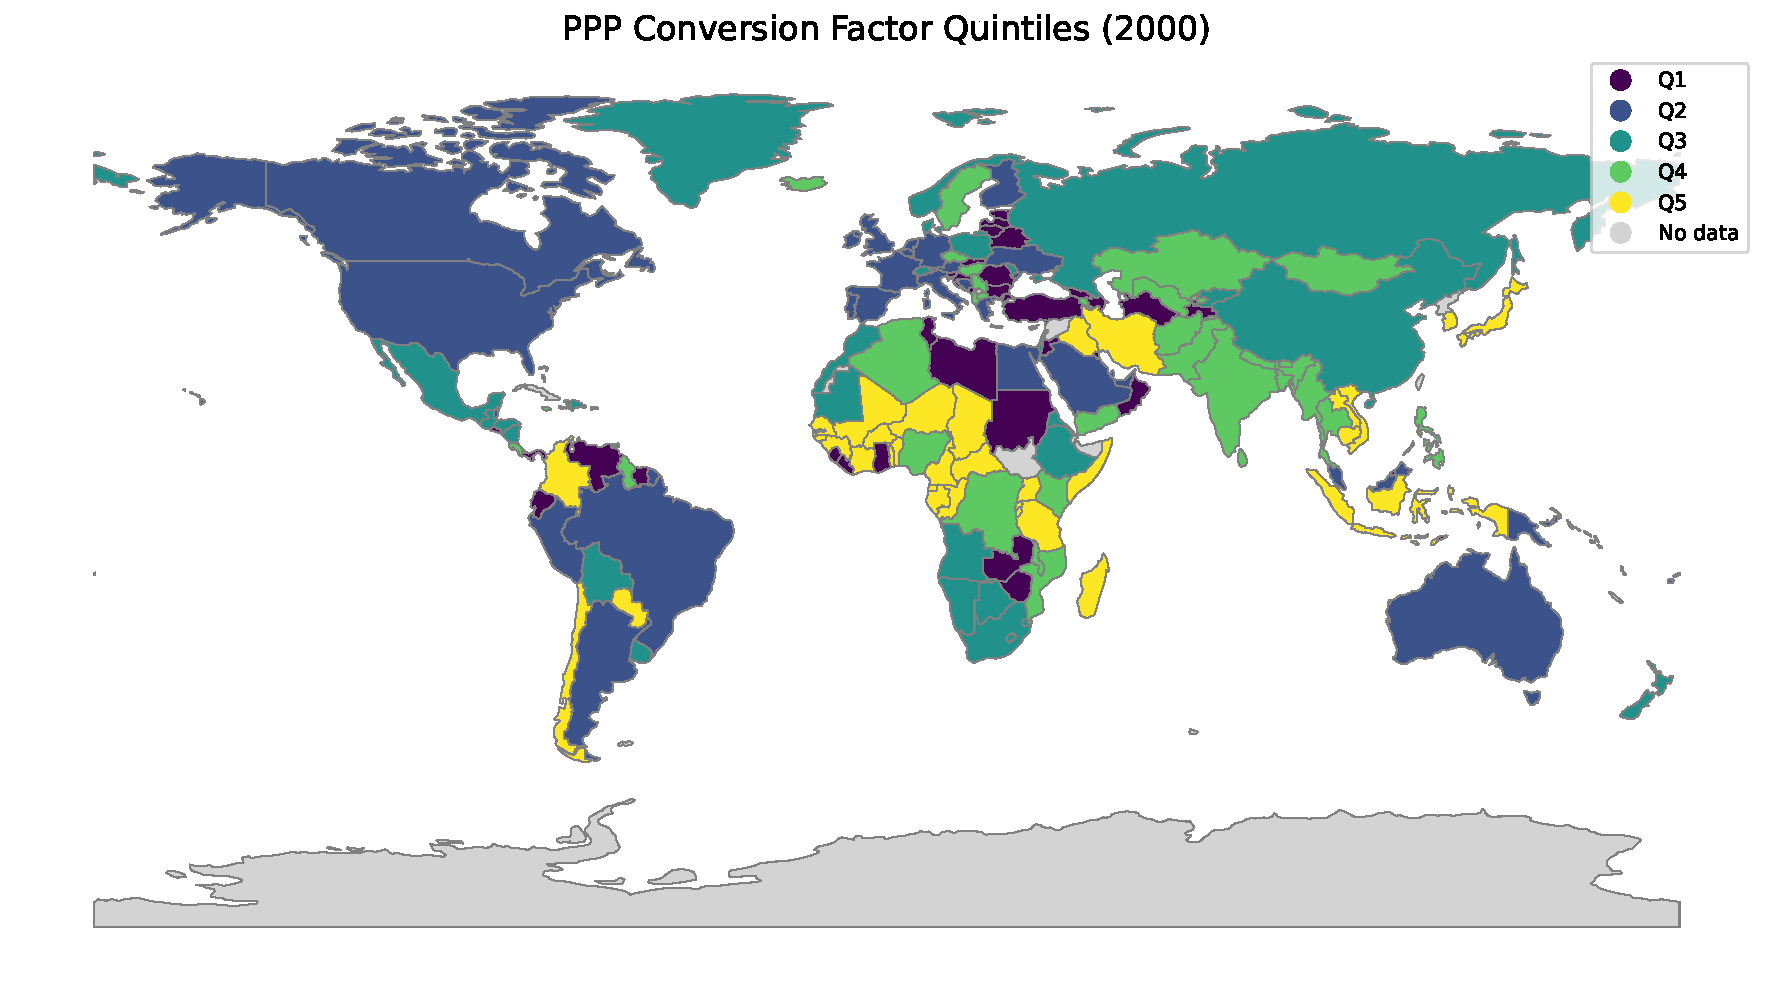
\includegraphics[width=0.9\linewidth]{figs/PPP_world_map_quintiles.pdf}
    \end{figure}
\end{frame}


\begin{frame}{A modern take...}
\begin{wideitemize}
    \item There are two main problems with all of the papers we have seen so far

    \item <2->First, none of them rely on a true multi-country model to know what to test
    \begin{itemize}
        \item Only modern papers that came out after Eaton Kortum (2002) were able to do that 
    \end{itemize}

    \item<3-> Second, they do not deal with the selection effect:
    \begin{itemize}
        \item Don't observe the productivity of goods that a country does not produce
        \item Only observe productivity of goods productive enough to be produced
    \end{itemize}
    
\end{wideitemize}

\end{frame}


\begin{frame}{Latent productivities}
\begin{wideitemize}
    \item Let $a_i^k(g)$ be the unit labor requirement of good $g$ of industry $k$ in country $i$

    \item<2-> Average unit labor requirements of a country would be: 

    \begin{equation*}
        \bar{a}_i^k \equiv \frac{1}{N} \sum_g  a_i^k(g)
    \end{equation*}

    \item<3-> But if country $i$ only produces goods up to $G < 1$ (as in the DFS model we saw) average \blue{observed} unit labor requirements would be:

        \begin{equation*}
        \tilde{a}_i^k \equiv \frac{1}{N_G} \sum_g  a_i^k(g) \qquad \text{for } g \le G  
    \end{equation*}

    \item<4-> In general $\tilde{a}_i^k \le \bar{a}_i^k$, since these are by definition the most productive products

    
\end{wideitemize}

\end{frame}

\begin{frame}{Costinot, Donaldson and Komunjer (2012)}
\begin{wideitemize}
    \item Costinot, Donaldson and Komunjer (CDK, 2012) extend the multi-country Ricardian model to multiple industries

    \item<2-> They show, under some assumptions, we can map unobserved productivities to observed productivities

    \item<3-> Specifically, they show:

    \begin{equation*}
        \underbrace{\frac{\tilde{a}_i^k}{\tilde{a}_j^k}}_{\text{observed}} = \underbrace{\frac{\bar{a}_i^k}{\bar{a}_j^k}}_{\text{unobserved}} \times \underbrace{\left(\frac{1-\text{Import Share}_i^k}{1-\text{Import Share}_j^k}\right)^\theta}_{\text{observed}} 
    \end{equation*}

    \blue{Intuition}: more open economies (higher import shares) are able to avoid using their low productivity for some goods by importing these varieties.
    
\end{wideitemize}

\end{frame}




\begin{frame}{Estimating equation}
\begin{wideitemize}
    \item Now they have solved both issues:
    \begin{itemize}
        \item<2-> They have written a multi-country multi-sector Ricardian model and derived predictions; 
        \item<3-> They found a way to overcome the selection issue of non-observed productivities
    \end{itemize}
    \item<4-> They estimate the following equation:

    \begin{equation*}
    \ln \left( \frac{X_{i \to j}^k}{ 1-\text{Import Share}_i^k} \right) = \delta_{ij} + \delta^k_{i} - \theta \ln \tilde{a}_i^k + \varepsilon^k_{ij}
    \end{equation*}

    \noindent where:

    \begin{itemize}
        \item $X_{i \to j}^k$ are exports from $i$ to $j$ in industry $k$
        \item $\tilde{a}_i^k$ is the observed unit labor requirement
        \item $\delta_{ij}, \delta^k_{i}$ are bilateral and industry-source specific coefficients, that adjust for differences in pair-relationship (say, former colony) and industry characteristics (say, manufacturing vs services)
    \end{itemize}

    \item<5-> We expect $\theta > 0$
    
\end{wideitemize}

\end{frame}


\begin{frame}{Results are consistent with the Ricardian predictions}
    \begin{figure}
        \centering
        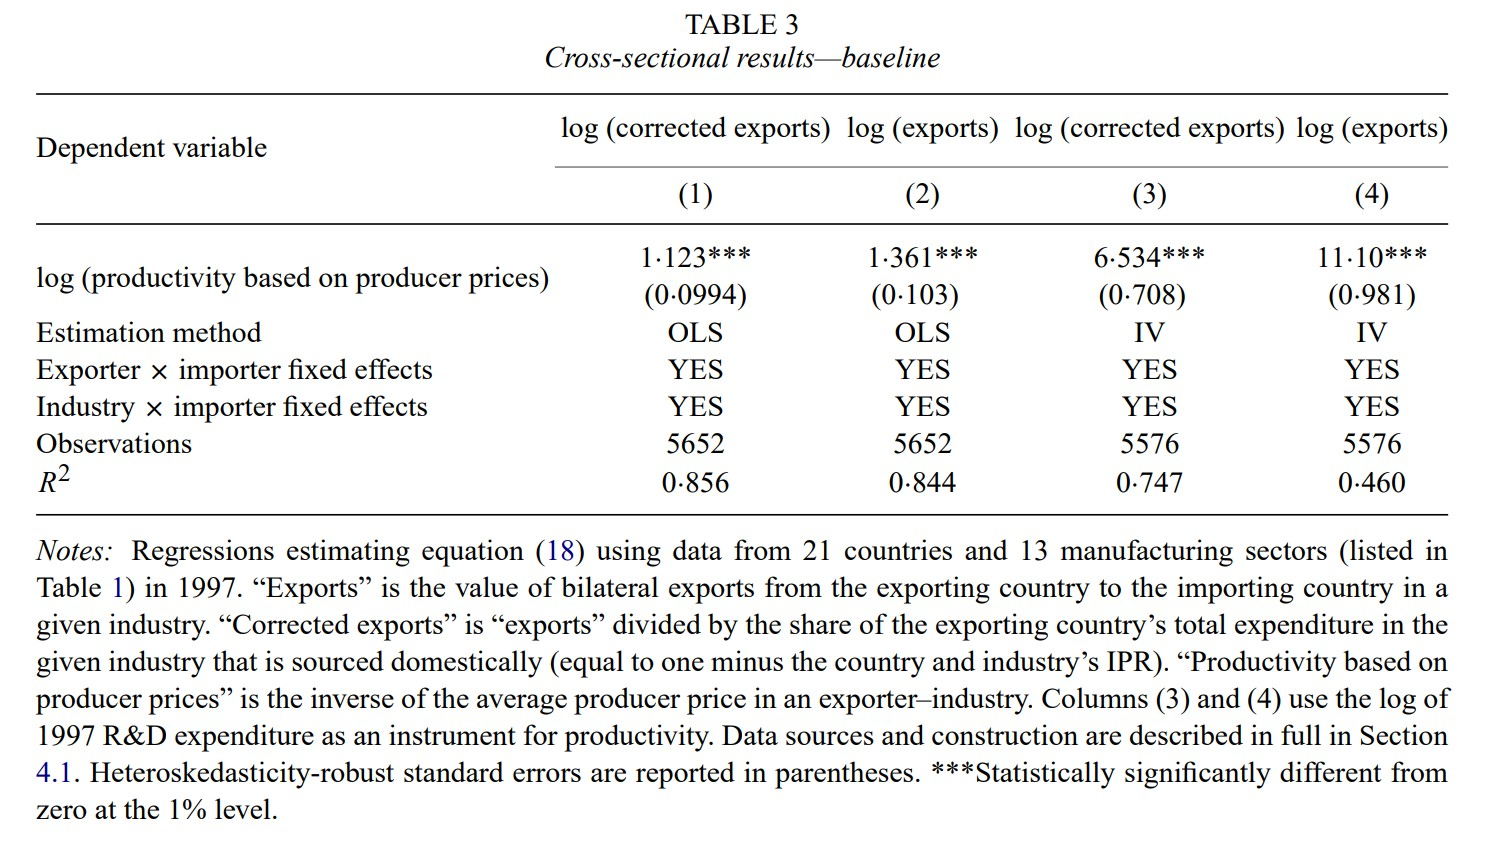
\includegraphics[width=0.6\linewidth]{figs/cdk1.jpg}
        \caption{Source: \href{https://academic.oup.com/restud/article/79/2/581/1532037}{Costinot, Donaldson and Komunjer (2012)} }
        \label{fig:cdk1}
    \end{figure}
\end{frame}

\begin{frame}{Results are consistent with the Ricardian predictions}
    \begin{figure}
        \centering
        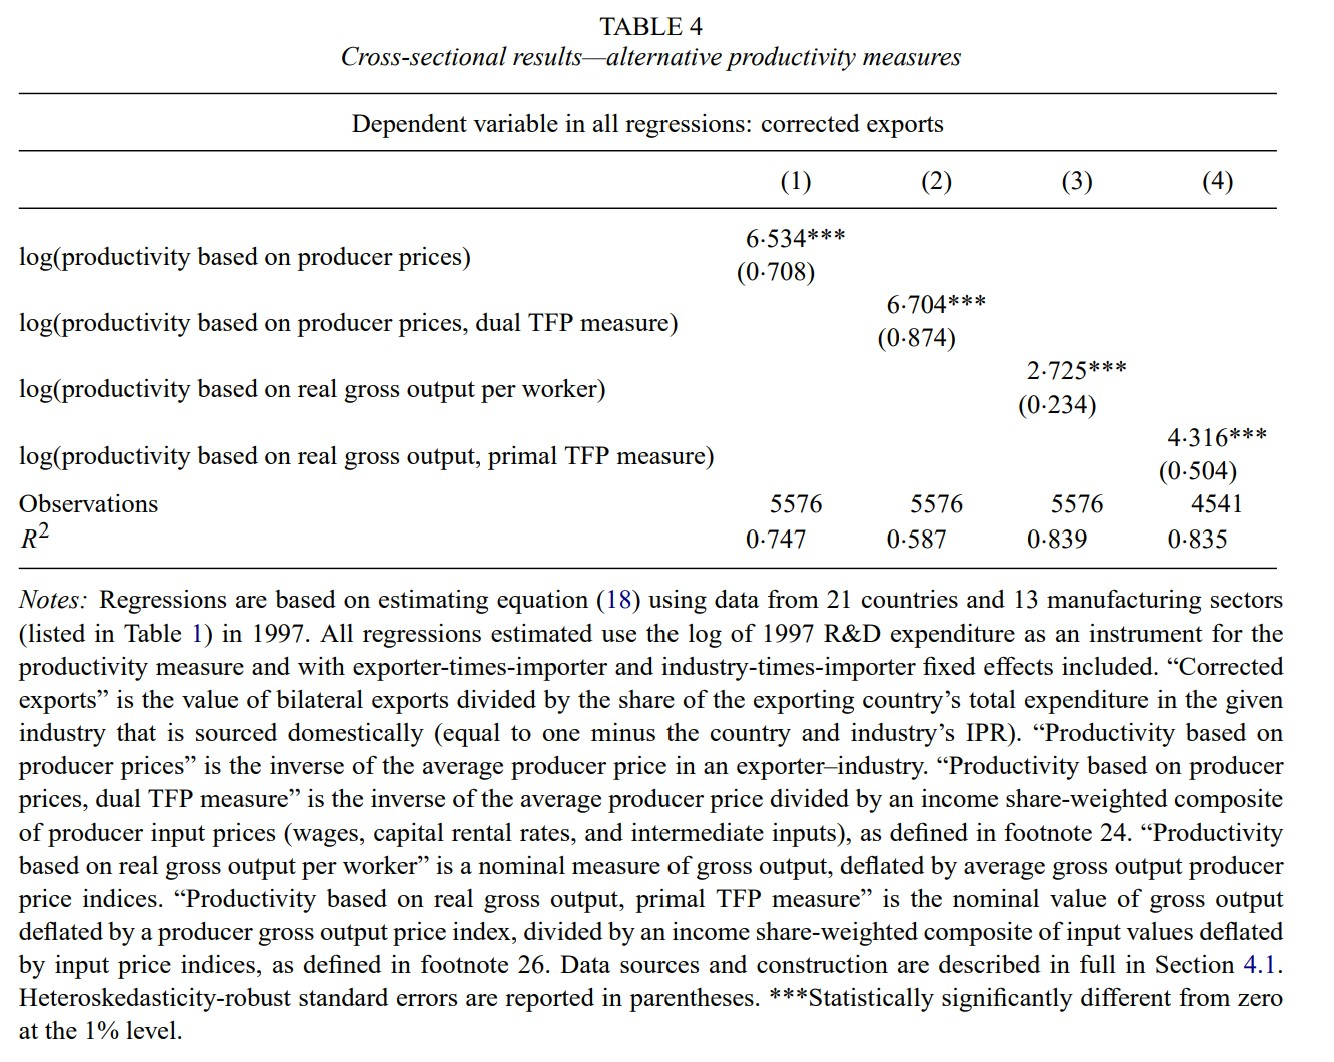
\includegraphics[width=0.6\linewidth]{figs/cdk2.jpg}
        \caption{Source: \href{https://academic.oup.com/restud/article/79/2/581/1532037}{Costinot, Donaldson and Komunjer (2012)} }
        \label{fig:cdk2}
    \end{figure}
\end{frame}

\begin{frame}{Takeaways}
\begin{wideitemize}
    \item We walked through the empirics of comparative advantage

    \item For the last 75 years, early and recent tests have confirmed important Ricardian intuitions

    \item More rigorous tests only happened surprisingly late

    \item Good example of theory + empirics being interdependent

    \item It was hard to reliably test the theory while it was underdeveloped
\end{wideitemize}
\end{frame}



\end{document}
